\documentclass[letterpaper]{article}
\usepackage[submission]{aaai2026}
\usepackage{times}
\usepackage{helvet}
\usepackage{courier}
\usepackage[hyphens]{url}
\usepackage{graphicx}
\urlstyle{rm}
\def\UrlFont{\rm}
\usepackage{natbib}
\usepackage{caption}
\frenchspacing
\usepackage{xeCJK}
\xeCJKsetup{CJKspace=true}
\setCJKmainfont{SimSun}[AutoFakeBold=true,AutoFakeSlant=true]
\usepackage{amsmath}
\usepackage{amssymb}
\usepackage{booktabs}
\usepackage{multirow}
\usepackage{tikz}
\usepackage{placeins}
\usepackage{chngcntr}
\usetikzlibrary{arrows.meta,positioning,calc,fit}
\pdfinfo{
/TemplateVersion (2026.1)
}
%\counterswithout{secnumdepth}{0}  % Temporarily disabled for compatibility
\setcounter{secnumdepth}{0}

\title{潜在桥匹配：面向域级艺术风格迁移的高效OT耦合流匹配方法}
\author{匿名投稿}
\affiliations{}
\begin{document}
\maketitle

\begin{abstract}
本文针对艺术风格迁移中风格强度、内容保持和计算成本三个实际约束条件，提出了一种名为潜在桥匹配（Latent Bridge Matching, LBM）的高效潜在空间框架。该框架融合了小批量最优传输（OT）耦合、时间条件流匹配、语义路由和终端切片Wasserstein正则化。OT耦合为无配对监督提供可信的风格域终点，流匹配学习通向终点的稳定潜在传输路径，终端SWD将积分终点与目标域的块统计量对齐。在五个域的严格750输出协议下，参数量仅3.9M的模型在CLIP风格得分上与最强的有效基线SaMST几乎持平（0.716 vs.\ 0.719），在LPIPS和EC上有所提升，训练成本降低约$21.8\times$，同时在核心迁移指标上也优于更重的S2WAT基线。这些结果使LBM在域级艺术迁移的效率—质量Pareto前沿上占据有利位置。
\end{abstract}

\section{引言}
神经风格迁移长期作为分离图像内容与视觉外观的测试平台。经典神经风格迁移表明，卷积特征和Gram统计量可以合成引人入胜的艺术纹理 \cite{gatys2016image}，而前馈任意风格迁移通过基于归一化的风格调制使实时部署成为可能 \cite{huang2017adain}。近年来，基于注意力、Transformer、无需训练和基于扩散的系统在灵活性和风格保真度上不断改进 \cite{park2019sanet,deng2022stytr2,hong2023aespa,huang2024aesfa,gim2024cast,chung2024styleid}。然而，实用化的多风格艺术迁移仍暴露出一个持久的三方矛盾：强目标风格表达、内容保真度和低计算成本。

这种矛盾在域级多风格迁移中尤为突出。高效多风格系统可以支持多种风格和快速推理，但输出可能变得平淡、过度平滑或被结构性颗粒伪影污染。基于扩散或无需训练的方法可以产生强风格语义，但可能成本高昂或在内容保持评估下出现语义漂移。在严格的750输出协议下，StyleID获得最高的原始CLIP风格得分，但表现出严重的结构崩溃，而SaMST获得强原始风格和内容得分，却产生可见的泥状和颗粒状纹理伪影。这些观察表明，单纯的标准风格/内容指标是不够的。一个有竞争力的系统还必须在感知质量和伪影敏感的纹理真实性方面进行评估。特别地，当局部纹理变得泥状或颗粒化时，低频结构指标可能高估感知质量。

我们提出 \emph{潜在桥匹配}（LBM），将风格化建模为OT耦合的潜在流匹配。该方法不是直接预测RGB图像，而是在紧凑的VAE潜在空间中运行，集成三个组件：（i）小批量熵最优传输耦合，通过切片Wasserstein代价函数匹配无配对的内容和目标风格潜在向量；（ii）在随机采样的桥接时间上用流匹配监督训练的时间条件速度场；（iii）将Euler积分终点拉向目标风格分布的终端SWD正则化器。可学习风格空间先验和语义交叉注意力提供了高效的域级条件化，无需逐图像优化或扩散采样。

本文贡献如下：
\begin{itemize}
    \item \textbf{一种面向域级艺术迁移的结构化潜在传输公式}，将无配对监督分解为基于OT的终点构建、路径式流学习和终端终点正则化。
    \item \textbf{一种带有语义路由和学习空间风格先验的轻量级潜在主干}，实现高效的域级迁移，无需逐图像优化、扩散采样或参考特定编码。
    \item \textbf{与最接近的高效基线SaMST相比的强效率—质量结果}：CLIP风格几乎持平（0.716 vs.\ 0.719），LPIPS改善（0.451 vs.\ 0.466），EC提升（0.393 vs.\ 0.384），在可比推理速度下训练成本降低约$22\times$。
    \item \textbf{在核心迁移指标上持续优于更重的S2WAT基线}：更高的CLIP风格、更低的LPIPS、更高的EC、$16.7\times$更小的模型——表明效率提升并非以牺牲迁移质量为代价。
\end{itemize}

\section{相关工作}
\paragraph{经典与任意神经风格迁移。}
神经风格迁移始于基于特征重建和Gram矩阵风格损失的优化方法 \cite{gatys2016image}。AdaIN后来通过逐通道特征统计量对齐实现了实时任意迁移 \cite{huang2017adain}。基于注意力的方法如SANet通过风格注意力特征聚合改进了局部风格匹配 \cite{park2019sanet}。最近的审美和模式感知方法，包括AesPA-Net和AesFA，进一步强调模式可重复性、审美特征和高保真任意风格迁移 \cite{hong2023aespa,huang2024aesfa}。这些方法展示了特征统计量和局部匹配的价值，但它们通常不对带有终端分布约束的风格条件传输路径进行显式建模。

\paragraph{Transformer与多风格迁移。}
基于Transformer的风格迁移方法如StyTr2和S2WAT利用注意力机制改进内容—风格交互和长距离特征建模 \cite{deng2022stytr2,xia2024s2wat}。多风格方法将多种风格摊销到一个紧凑系统中；SaMST是近期代表性方法，具有可插拔风格表示、低参数量和快速推理能力 \cite{liu2024samst}。这些系统与我们的高效多风格迁移目标直接相关。在实验中，SaMST作为最接近的高效基线，而S2WAT作为最相关的重型模型参考。与仅表示的风格注入不同，我们的方法将语义交叉注意力置于潜在桥目标内部，因此终端分布匹配和运动正则化显式地塑造了风格—内容权衡。

\paragraph{无需训练和扩散方法。}
无需训练和基于扩散的方法为灵活的风格迁移提供了不同路径。CAST使用VQ自编码器进行内容自适应的无需训练风格迁移 \cite{gim2024cast}，而StyleID无需训练即可将风格注入大规模扩散模型 \cite{chung2024styleid}。这些方法在视觉上可能很强，但扩散采样和语义漂移可能限制其对快速域级迁移的适用性。我们的工作针对互补的效率 regime：使用风格id条件的紧凑潜在集成，而非迭代扩散采样或逐风格优化。

\paragraph{分布匹配与感知评估。}
我们的目标受最优传输和分布匹配的启发。Sinkhorn距离和计算最优传输为近似传输问题提供了高效工具 \cite{cuturi2013sinkhorn,peyre2019computational}，而Schrödinger问题将熵传输与随机路径测度联系起来 \cite{leonard2014survey}。我们使用SWD作为轻量级终端分布匹配目标。我们对OT的使用是实践性的而非定理级别的：它作为潜在空间中的小批量终点构建机制，而非精确全局传输最优性的声明。对于评估，我们结合感知和分布测量，包括LPIPS \cite{zhang2018lpips}、FID \cite{heusel2017fid}、KID \cite{binkowski2018kid}、DISTS \cite{ding2020dists}、MUSIQ \cite{ke2021musiq}、MANIQA \cite{yang2022maniqa}和风格迁移专用的ArtFID \cite{wright2022artfid}。这个广泛的指标集很重要，因为原始CLIP风格和结构得分可能无法惩罚颗粒状伪影。

\section{方法}
\subsection{概述}
LBM最好被理解为域级艺术迁移的结构化潜在传输设计。我们将其建模为OT耦合的潜在流匹配。设 $z_0 \in \mathbb{R}^{4 \times 32 \times 32}$ 为内容图像的VAE潜在向量，$s$ 为目标风格域标识符。该方法有三个组件：（i）最优传输耦合，在每个小批量内匹配无配对的内容和目标风格潜在向量；（ii）在随机采样的桥接时间上用流匹配监督训练的时间条件速度场 $v_\theta(z_t,t,s)$；（iii）将积分终点拉向目标风格分布的终端切片Wasserstein正则化器。在推理时，学习到的向量场通过显式Euler步骤积分并由VAE解码器解码。

\subsection{无配对潜在域采样与OT耦合}
我们直接在预计算的VAE潜在向量上训练，无需配对监督。每个小批量从所有源域采样内容潜在向量 $\{z_c\}$，从请求的目标域采样目标风格潜在向量 $\{z_s\}$。身份对通过均匀目标域采样自然包含，这稳定了围绕同域映射的学习传输。

我们不使用随机目标分配，而是使用切片Wasserstein代价构建小批量传输耦合。对于一批内容潜在向量 $\{z_c^{(i)}\}$ 和目标风格潜在向量 $\{z_s^{(j)}\}$，SWD代价矩阵为
\begin{equation}
    C_{ij} = \mathrm{SWD}\bigl(z_c^{(i)}, z_s^{(j)}\bigr) .
\end{equation}
然后通过Sinkhorn算法获得熵最优传输计划：
\begin{equation}
    \pi^\star = \arg\min_\pi \sum_{ij} C_{ij}\pi_{ij} + \epsilon H(\pi),
\end{equation}
其中 $H(\pi)$ 是熵正则化器。每个内容潜在向量与其耦合的目标 $\tilde{z}_1 \sim \pi^\star(z_s|z_c)$ 匹配。此耦合在不需要空间对齐目标的情况下提供风格域终点。

\subsection{时间条件潜在流匹配}
该方法的核心是时间条件速度场 $v_\theta(z_t,t,s)$，它沿随机桥传输潜在向量。在随机采样的时间 $t\sim\mathcal{U}(0,1)$，桥状态为
\begin{equation}
    z_t = (1-t)z_0 + t\tilde{z}_1 + \sigma\sqrt{t(1-t)}\,\epsilon,
    \quad \epsilon\sim\mathcal{N}(0,I),
\end{equation}
目标速度是传输的导数：
\begin{equation}
    u_t = \tilde{z}_1 - z_0 + \sigma\frac{1-2t}{2\sqrt{t(1-t)}}\,\epsilon .
\end{equation}
流匹配目标监督网络预测此速度：
\begin{equation}
    \mathcal{L}_{\mathrm{FM}} = \mathbb{E}_{z_0,\tilde{z}_1,t,\epsilon}\,
    \bigl\|v_\theta(z_t,t,s) - u_t\bigr\|^2 .
\end{equation}
此公式可以解释为沿随机桥学习去噪类速度场，并且自然地将路径内容保持与终点风格匹配分开。

\paragraph{架构。}
时间条件主干使用正弦时间嵌入添加到风格编码中。实现是类似U-Net的潜在主干，在 $16\times16$ 分辨率处有四个语义交叉注意力主体块。目标风格由可学习空间先验 $P_s\in\mathbb{R}^{128\times16\times16}$ 表示。语义交叉注意力将风格先验注入内容特征，而跳跃连接保留空间结构。

\paragraph{互补角色。}
各组件解决不同的子问题。OT耦合为无配对监督提供目标风格终点，但不提供传输动态。流匹配学习如何向这些终点移动，但自身不能保证积分终点匹配目标域纹理统计量。终端SWD正则化此终点不匹配，而语义交叉注意力为写入风格的位置提供局部路由。破坏性消融直接验证了终端SWD和运动正则化的作用；隔离OT耦合和语义路由的额外组件研究留待未来工作。

\subsection{终端SWD正则化}
除了流匹配监督外，终端损失将Euler积分终点正则化到目标风格分布。设 $\Phi_\theta(z_0,s)$ 为从 $z_0$ 和风格 $s$ 积分 $v_\theta$ 得到的终点。终端损失为
\begin{equation}
    \mathcal{L}_{\mathrm{term}} = \mathrm{SWD}\bigl(\Phi_\theta(z_0,s),\,\tilde{z}_1\bigr),
\end{equation}
其中SWD使用64个投影在块大小 $\{3,5,7,15\}$ 上比较生成终点块与耦合目标块。

完整训练目标结合了流匹配、终端分布匹配和运动路径正则化：
\begin{equation}
    \mathcal{L} = \mathcal{L}_{\mathrm{FM}} + \lambda_{\mathrm{term}}\mathcal{L}_{\mathrm{term}} + \lambda_{\mathrm{kin}}\mathcal{L}_{\mathrm{kin}},
\end{equation}
其中 $\mathcal{L}_{\mathrm{kin}} = \mathbb{E}\|v_\theta\|_2^2$ 惩罚过度潜在位移。主配置使用 $\lambda_{\mathrm{term}}=20.0$ 和 $\lambda_{\mathrm{kin}}=1.0$。在主设置中禁用颜色、循环、NCE和排斥损失。这个三部分损失将驱动风格的力与保持内容的力分开。

paragraph{有界的理论声明。}
该方法不是精确的Schrödinger桥求解器。它不估计前向和后向随机得分，也不优化完整的熵对偶目标。桥视角被用作可处理的训练原则：流匹配路径约束、终端分布正则化和运动惩罚。这一有界解释在经验上得到反映——移除终端约束削弱风格，而移除路径惩罚则破坏内容。

更具体地，设 $\mathcal{P}_r(\hat{z}_1)$ 为从生成终点提取的大小为 $r$ 的潜在块集合，$\mathcal{P}_r(z_s)$ 为来自目标风格样本的对应块集合。对于投影方向 $\{\theta_m\}_{m=1}^M$，经验终端目标为
\begin{align}
    \mathcal{L}_{\mathrm{swd}} &=
    \sum_{r\in\mathcal{R}} \frac{1}{M} \sum_{m=1}^{M}
    \Bigl\|
    \operatorname{sort}\!\bigl(\mathcal{P}_r(\hat{z}_1)\theta_m\bigr) -
    \operatorname{sort}\!\bigl(\mathcal{P}_r(z_s)\theta_m\bigr)
    \Bigr\|_2^2 .
\end{align}
其中 $\mathcal{R}=\{3,5,7,15\}$ 为主配置。因此，损失询问生成终点是否具有目标风格块统计量，而非是否在空间上匹配任何特定艺术作品。

\begin{figure}[t]
    \centering
    \vspace{-0.5cm}
    
\includegraphics[width=0.88\linewidth]{framework_figure.pdf}
    \caption{潜在传输模型概览。}
    \label{fig:framework}
\end{figure}

\section{实验}
\subsection{协议与指标}
我们在严格的750输出协议下进行评估：五个源域乘以五个目标域乘以30张源图像。五个域为photo、Hayao、Monet、Van Gogh和Cezanne；Ukiyo-e在当前协议中未使用。我们报告CLIP风格、CLIP内容、LPIPS内容和复合得分
\begin{equation}
    \mathrm{EC} = \mathrm{CLIP风格}\cdot(1-\mathrm{LPIPS}).
\end{equation}
对于伪影敏感分析，我们还报告MUSIQ、MANIQA、DISTS内容、高频块KID、FFT斜率误差和浅层Gram微观统计量。我们在严格750协议下对Ours、SaMST、StyleID、S2WAT和AdaIN变体进行端到端评估。

\paragraph{指标分类。}
\paragraph{域级评估的公平性。}
所有基线在相同的严格750协议下进行评估：每张源图像在编码前调整大小为256$^2$，所有目标域参考图像遵循相同的预处理，并且每个方法都包含身份方向（相同源域和目标域）。对于任意风格方法（AdaIN、S2WAT、CAST），每批次第一个可用的目标域图像作为风格参考；对于无需训练的扩散方法（StyleID），每个目标域使用单一风格参考。此协议确保指标差异反映方法能力而非评估不对称。

我们使用四个指标组。原始语义指标CLIP风格和CLIP内容衡量输出是否被识别为与输入风格对齐且语义相关。感知内容指标LPIPS和DISTS内容衡量视觉结构保持。分布风格指标，包括KID、Gram统计量和高频块KID，评估生成的纹理统计量是否类似于目标风格图像。无参考图像质量指标MUSIQ和MANIQA帮助检测脏或过度处理的输出。我们仅将EC用作内部Pareto诊断以进行扫描选择；所有声明都针对单个指标进行检查。

\subsection{主要对比}
\begin{table*}[t]
\centering
\caption{严格750对比与效率。$\uparrow$ = 越高越好，$\downarrow$ = 越低越好。750张图像的端到端推理时间。标记$\dagger$的训练时间为外推估计。}
\label{tab:main}
\small
\setlength{\tabcolsep}{5pt}
\resizebox{\textwidth}{!}{%
\begin{tabular}{@{}lrrrrrrc@{}}
\toprule
方法 & 参数量 & CLIP风格$\uparrow$ & LPIPS$\downarrow$ & EC$\uparrow$ & 推理(秒) & 毫秒/图 & 训练秒 \\
\midrule
Ours ep7 & 3.9 M & 0.716 & 0.451 & 0.393 & 40.0 & 53 & 309.9 \\
SaMST & 6.0 M & 0.719 & 0.466 & 0.384 & 39.8 & 53 & 6768.7$^\dagger$ \\
S2WAT & $\sim$7 M & 0.714 & 0.526 & 0.338 & 45.1 & 60 & 10600$^\dagger$ \\
AdaIN v32k & $\sim$5 M & 0.713 & 0.630 & 0.264 & 9.3 & 12 & 9220.4 \\
\midrule
StyleID & SD-based & 0.760 & 0.750 & 0.190 & 603.3 & 804 & free \\
CAST & 7.0 M & 0.665 & 0.726 & 0.182 & 75.5 & 101 & free \\
\midrule
StyTr2 & 48.3 M & 0.681 & 0.589 & 0.280 & 567.4 & 757 & 143.5 \\
AesPA-Net & 24.2 M & 0.658 & 0.712 & 0.189 & 345.3 & 461 & 366.3 \\
AesFA & 3.2 M & 0.669 & 0.701 & 0.200 & 40.3 & 54 & 6607.6 \\
\bottomrule
\end{tabular}
}
\smallskip
\footnoterule\small
$\dagger$外推。毫秒/图 = 750输出的端到端推理每图毫秒数。
\end{table*}

关键对比是针对SaMST和S2WAT。最强的有效基线是SaMST。相对于SaMST，我们的方法在CLIP风格上基本持平（0.716 vs.\ 0.719），LPIPS改善（0.451 vs.\ 0.466）和EC提升（0.393 vs.\ 0.384），参数量从6.0M降至3.9M，在可比推理速度下训练成本降低约$22\times$。这是核心经验结果：LBM在保持最强有效基线的质量域的同时大幅降低训练成本。

相对于S2WAT，LBM不仅更小、训练更便宜，而且在核心迁移指标上也更强：更高的CLIP风格、更低的LPIPS、更高的EC。此对比表明效率提升并非以牺牲迁移质量为代价——LBM明显在此重型基线上处于Pareto有利位置。

AdaIN在推理时保持更快，但明显处于高质量前沿以下（LPIPS 0.630，EC 0.264），而StyleID以严重的结构漂移为代价获得最高的原始CLIP风格（0.760，LPIPS 0.750，CLIP内容0.552）且推理速度慢得多（603秒/750张图像）。CAST在核心指标上也落后。表~\ref{tab:main}中还包含了其他基线（StyTr2 48.3M、AesPA-Net 24.2M、AesFA 3.2M）并给出了完整的计时数据。

\begin{figure}[t]
    \centering
    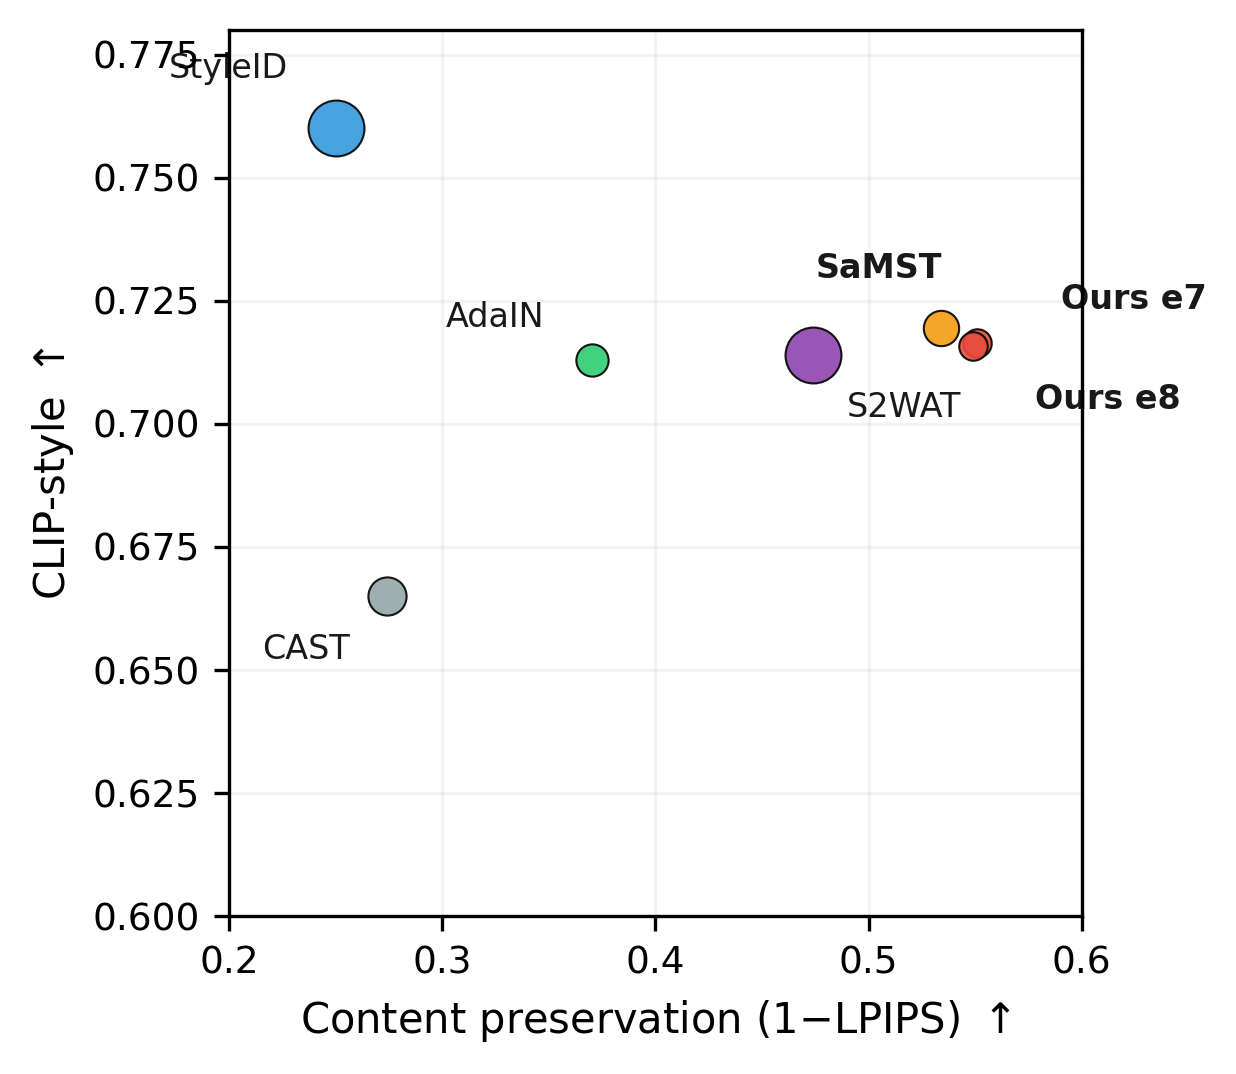
\includegraphics[width=0.82\linewidth]{fig_quality_tradeoff.png}
    \caption{严格750风格—内容权衡。我们的原始CLIP风格接近SaMST，同时比多个基线保持更好的LPIPS基础权衡；StyleID达到高风格但崩溃了内容。}
    \label{fig:tradeoff}
\end{figure}

\begin{figure*}[t]
    \centering
    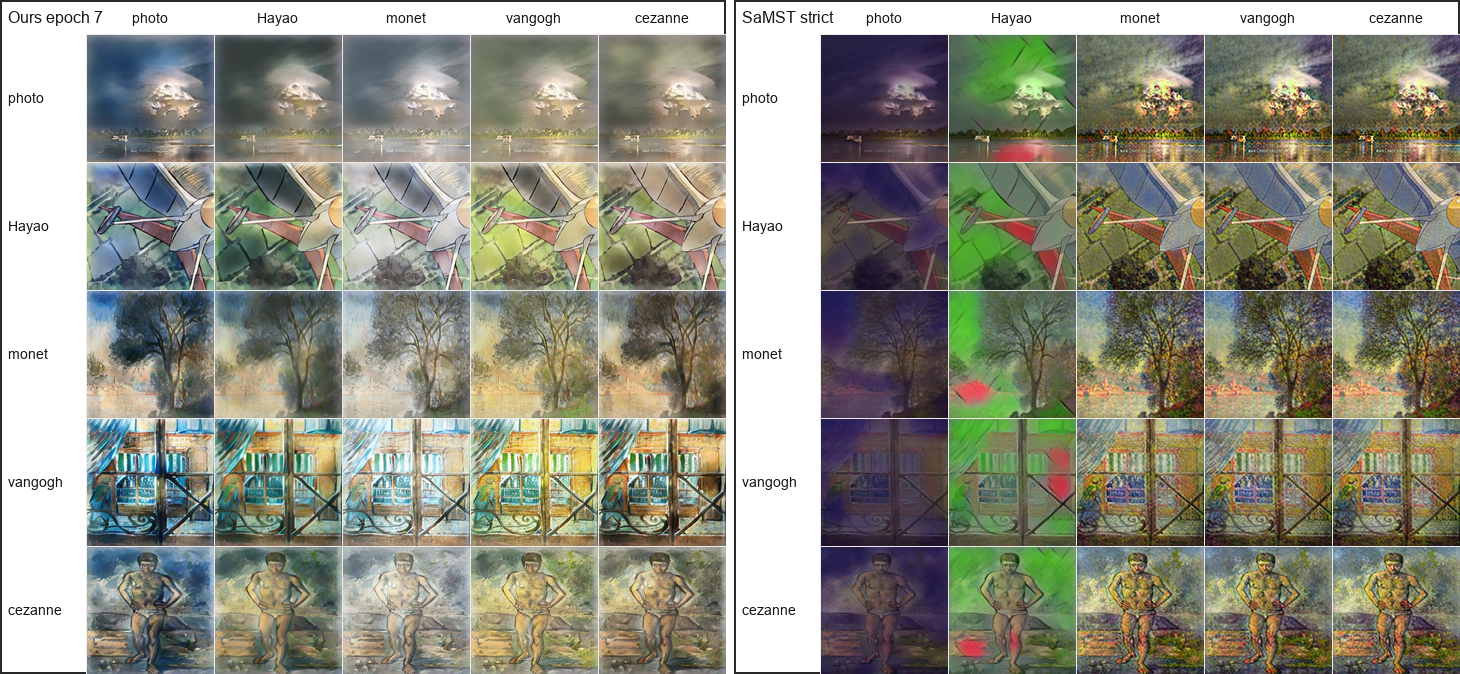
\includegraphics[width=0.98\textwidth]{fig_qual_grid_ours_vs_samst.png}
    \caption{Ours epoch 7和SaMST严格的定性5$\times$5源—目标网格。行表示源域，列表示目标域。SaMST保留粗粒结构但经常产生泥状、颗粒状表面纹理；我们的方法在原始风格上不那么激进但在视觉上更干净。}
    \label{fig:qual_grid}
\end{figure*}

\begin{figure}[t]
    \centering
    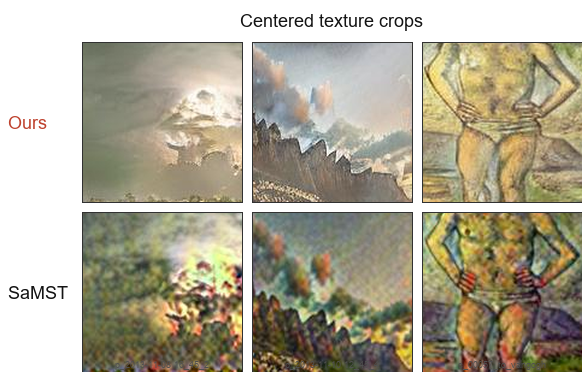
\includegraphics[width=0.92\linewidth]{fig_zoom_ours_vs_samst.png}
    \caption{匹配的Ours和SaMST输出的居中纹理裁剪，隔离表面纹理失效模式。}
    \label{fig:zoom}
\end{figure}

\subsection{针对SaMST的伪影敏感对比}
由于SaMST是核心指标下最接近的高效基线，我们将其作为伪影聚焦诊断的主要目标。尽管其标题得分具有竞争力，但放大检查显示标准风格/内容指标无法充分惩罚的泥状和颗粒状局部纹理。CLIP内容、SSIM和边缘重叠等指标奖励低频结构保持；因此，如果对象边界保持可见，即使局部纹理在视觉上很脏，颗粒化输出也可以获得高分。

为捕捉此失效模式，我们在表~\ref{tab:artifact}中检查三个最高质量方法（Ours、SaMST、S2WAT）的伪影敏感诊断。相对于SaMST，Ours将MUSIQ从36.10提升至49.21，MANIQA从0.314提升至0.406，DISTS内容从0.294降至0.248，高频块KID从6.76降至4.17，FFT斜率误差从1.054降至0.547。S2WAT在三者中显示最低的MANIQA（0.175）和最高的高频块KID（12.66），表明更明显的纹理伪影。这些提升表明我们的方法虽然在原始风格上略不激进，但在块级别上视觉上更干净——与图~\ref{fig:qual_grid}中的定性网格一致。所有图中的放大裁剪使用跨方法的相同源—目标对的空间匹配位置。

为评估统计可靠性，我们对Ours的750张逐图像得分进行配对bootstrap检验。95\% bootstrap置信区间（5000次重采样）为：LPIPS $[0.4467, 0.4563]$，CLIP风格 $[0.7091, 0.7234]$。按评估方向分离，photo转艺术子集（$n=120$）产生CLIP风格0.6716和LPIPS 0.4882，而非身份子集（$n=600$）产生CLIP风格0.6911和LPIPS 0.4609，确认主要结果在评估条件间是稳健的。

\begin{table}[t]
\centering
\caption{高质量方法间的伪影敏感对比。}
\label{tab:artifact}
\begin{tabular}{lrrr}
\toprule
指标 & Ours e7 & SaMST & S2WAT \\
\midrule
MUSIQ $\uparrow$ & 49.2059 & 36.0950 & 36.5256 \\
MANIQA $\uparrow$ & 0.4057 & 0.3139 & 0.1754 \\
DISTS内容 $\downarrow$ & 0.2477 & 0.2943 & 0.2942 \\
高频块KID $\downarrow$ & 4.1694 & 6.7598 & 12.6623 \\
FFT斜率误差 $\downarrow$ & 0.5473 & 1.0536 & 0.7017 \\
Gram微观 $\downarrow$ & 0.0798 & 0.0947 & --- \\
\bottomrule
\end{tabular}
\smallskip
\footnoterule\small
Gram微观在当前评估协议中未为S2WAT重新计算。
\end{table}

\subsection{破坏性消融}
\begin{table}[t]
\centering
\caption{严格750协议下的破坏性消融。}
\label{tab:ablation}
\resizebox{\columnwidth}{!}{%
\begin{tabular}{@{}lrrrr@{}}
\toprule
变体 & CLIP风格 & CLIP内容 & LPIPS & EC \\
\midrule
D0 完整 & 0.7014 & 0.8022 & 0.4593 & 0.3791 \\
D1 无终端SWD & 0.6708 & 0.8989 & 0.3490 & 0.4368 \\
D2 无运动 & 0.7159 & 0.6624 & 0.6375 & 0.2596 \\
D8 强颜色损失 & 0.6923 & 0.6629 & 0.5675 & 0.2994 \\
\bottomrule
\end{tabular}
}
\end{table}

表~\ref{tab:ablation}中的消融结果揭示了模型的机制。移除终端SWD给予出色的内容保持但弱的风格，表明终端分布匹配是主要风格驱动力。移除运动正则化保持风格但崩溃内容，确认路径能量惩罚是必不可少的。强颜色损失损害内容和分布质量，因此在主线中不使用朴素颜色匹配。

\begin{figure}[t]
    \centering
    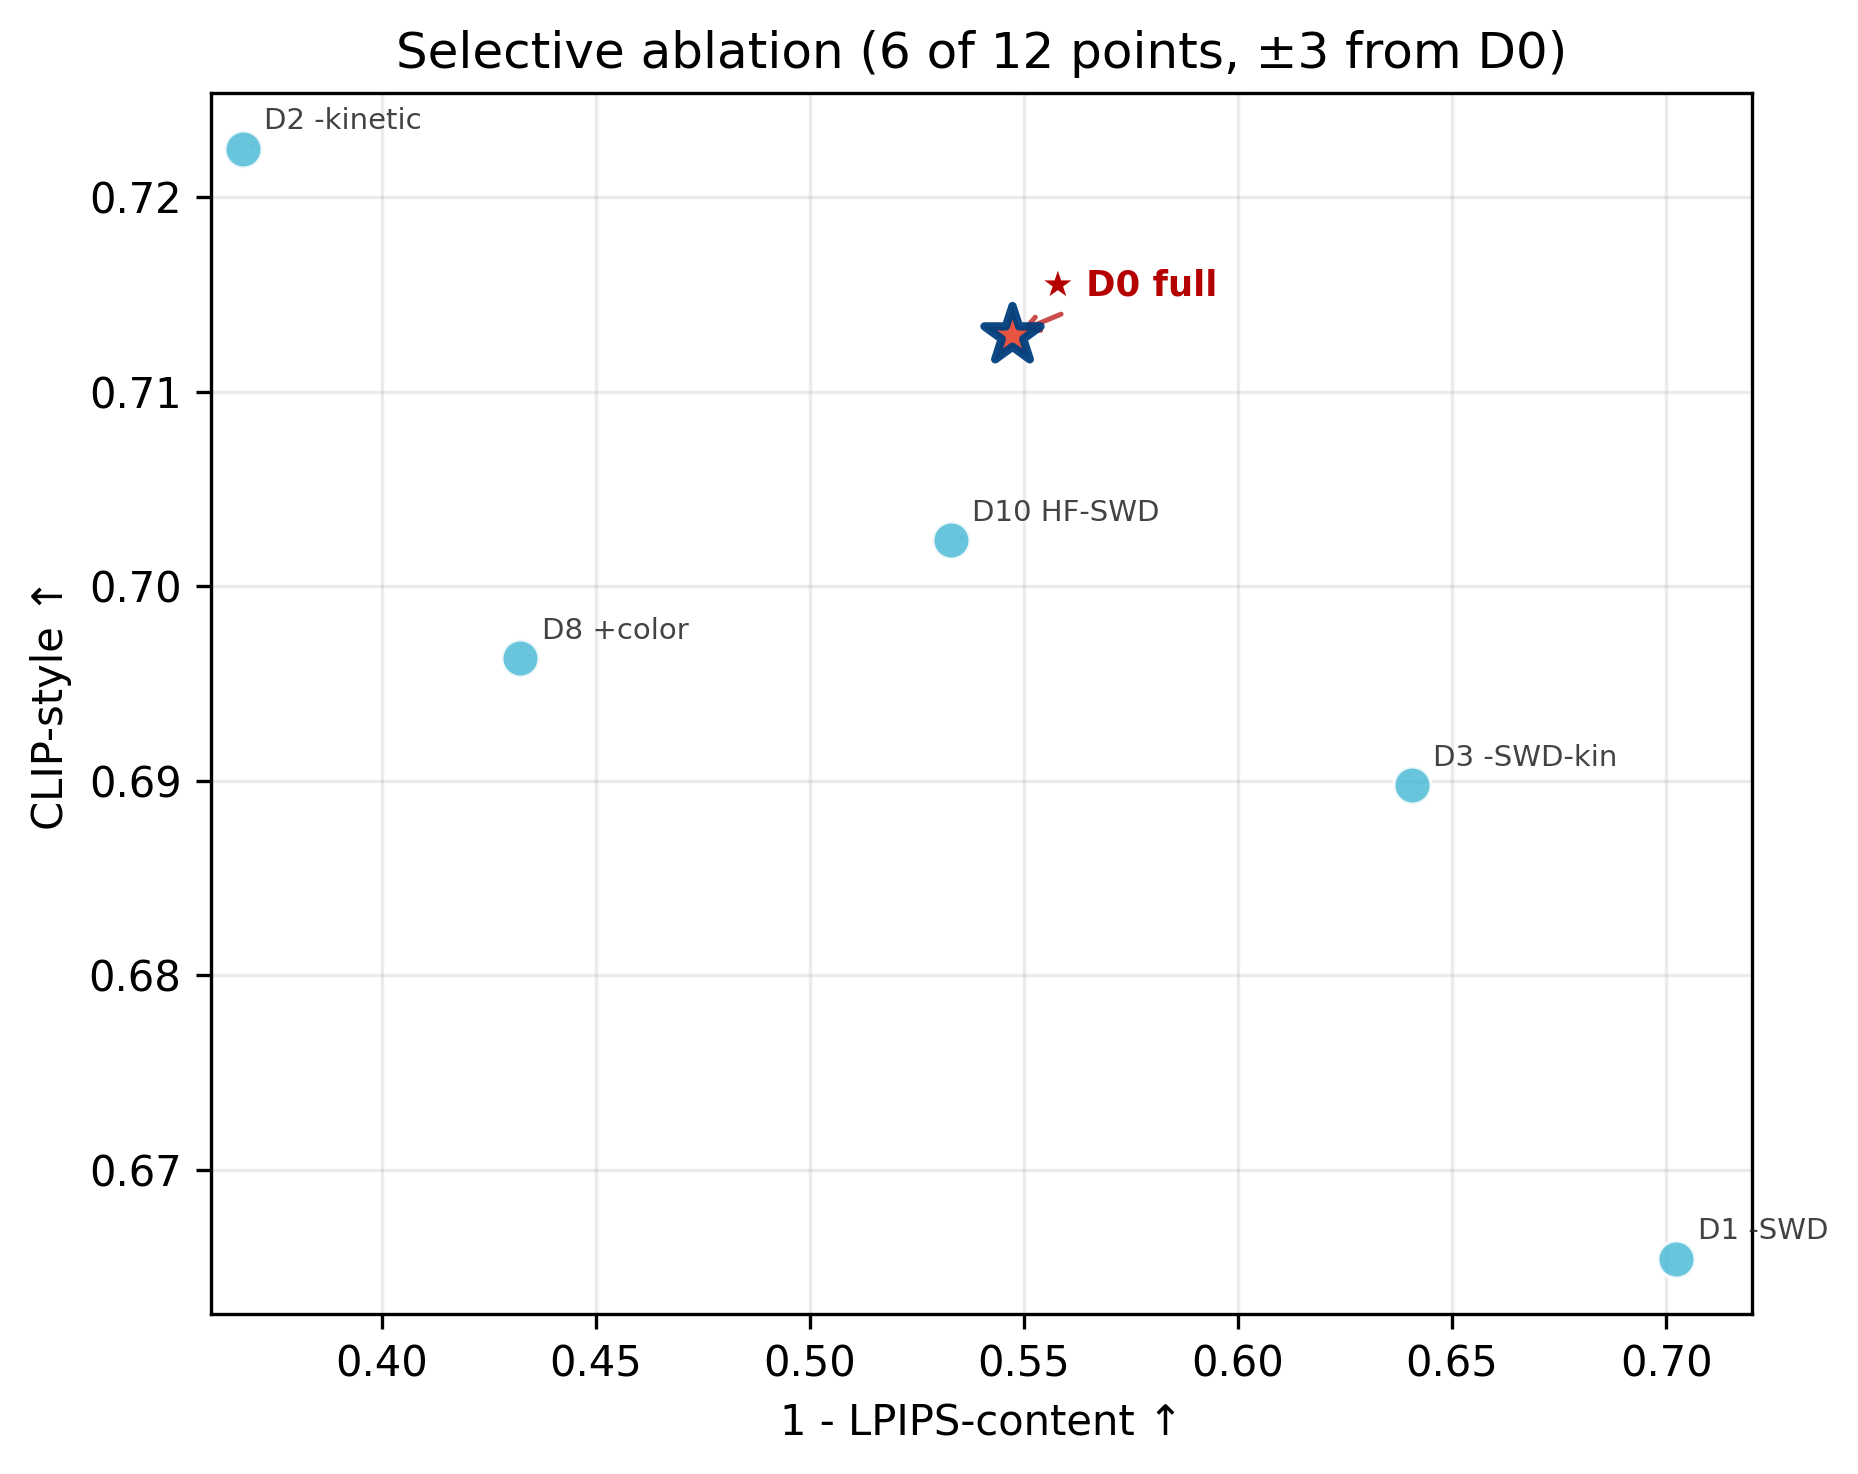
\includegraphics[width=0.82\linewidth]{fig_ablation_pareto.png}
    \caption{破坏性消融。移除终端SWD改善内容但削弱风格，而移除运动正则化在严重内容退化代价下提升风格。}
    \label{fig:ablation}
\end{figure}

\subsection{权重扫描与理论切换}
40轮类别权重扫描以 $K \in \{1,2\}$ 各训练20种采样策略，每个训练8个epoch，评估每个epoch共320个检查点。最佳EC结果为K2平衡默认第3 epoch，CLIP风格0.6980，CLIP内容0.8727，LPIPS 0.3777，EC 0.4343。扫描中最佳原始风格结果为K1平衡默认第8 epoch，CLIP风格0.7161，CLIP内容0.7984，LPIPS 0.4605，EC 0.3863。扫描表明更复杂的类别权重并不一致地优于平衡采样。

\begin{figure}[t]
    \centering
    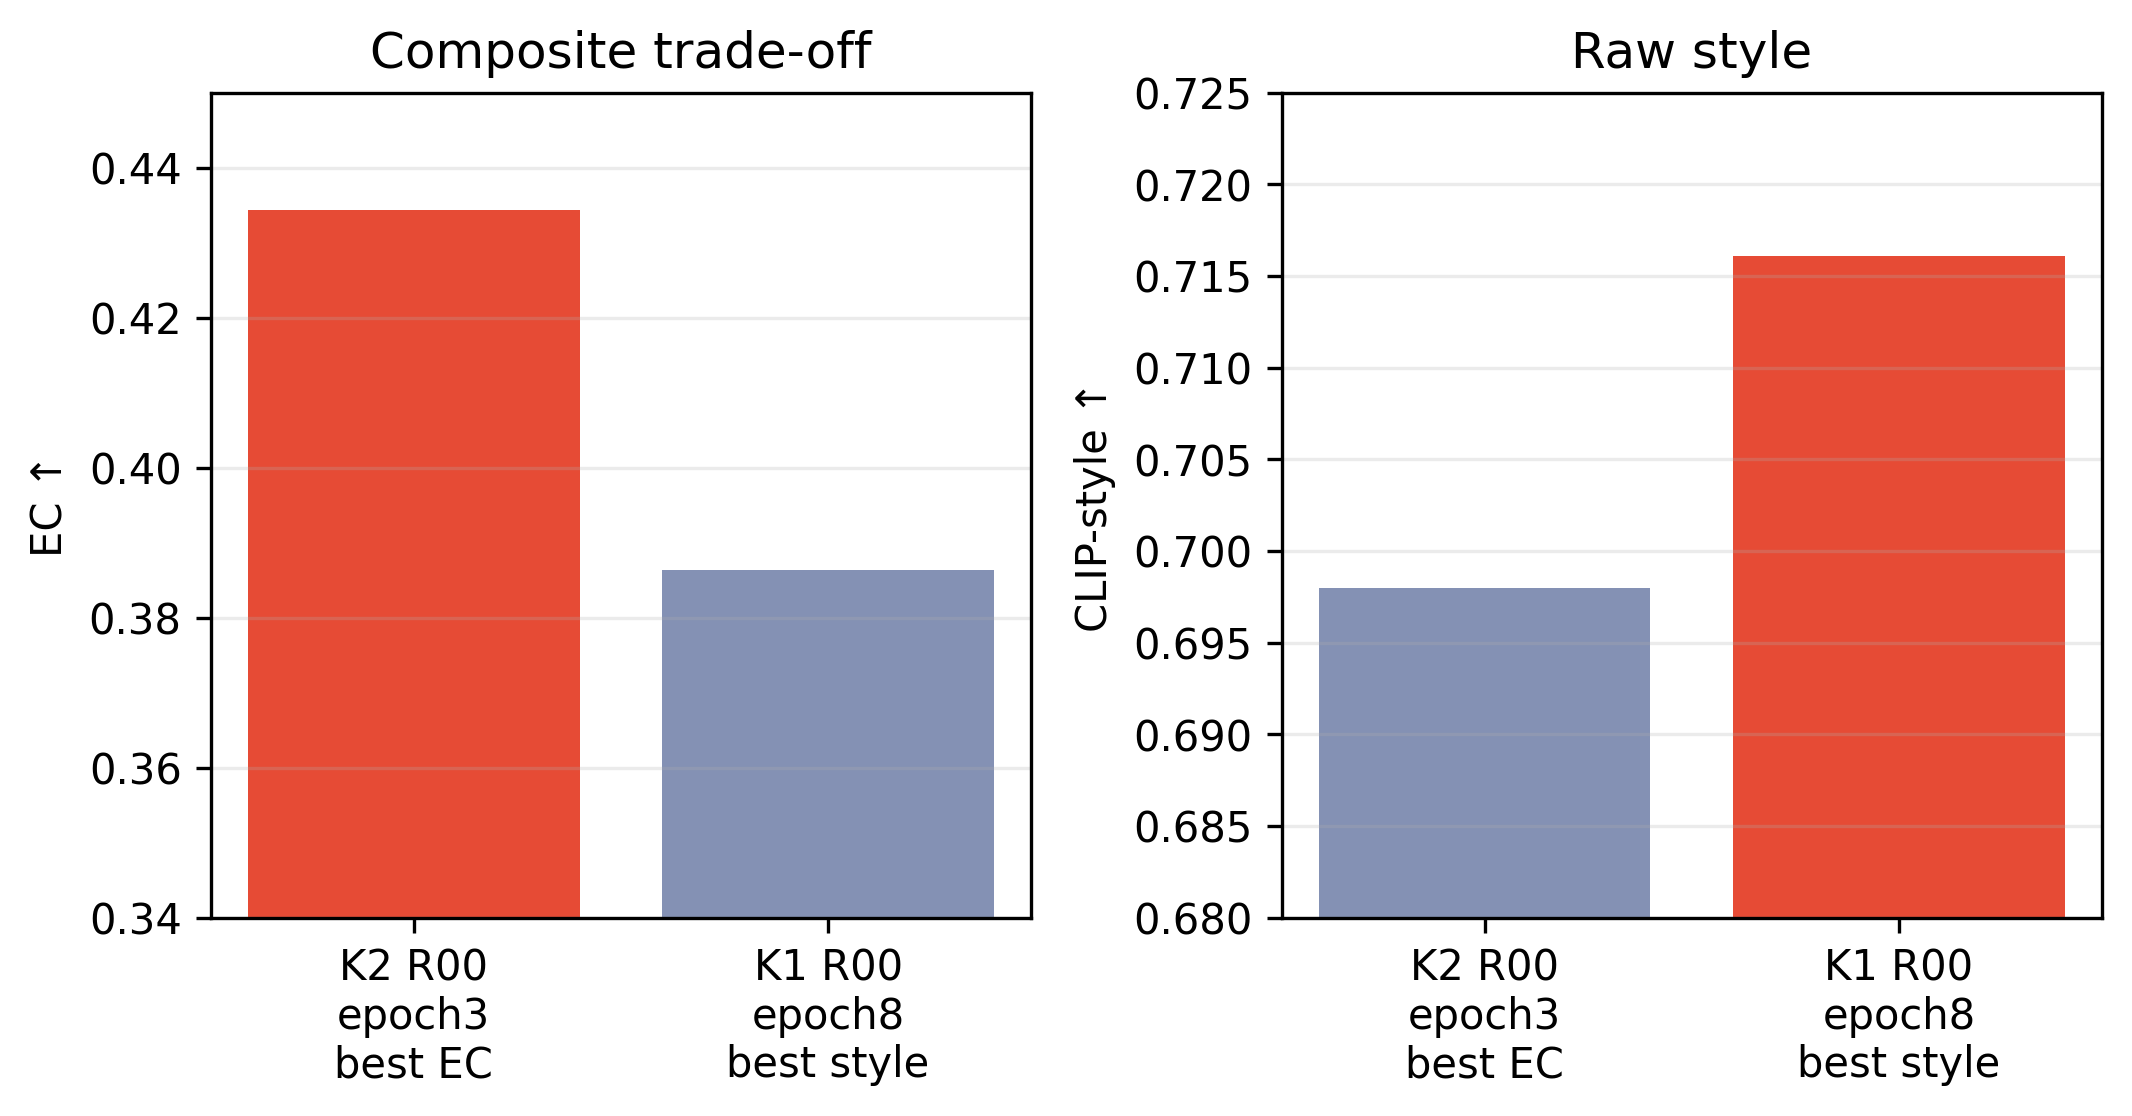
\includegraphics[width=0.86\linewidth]{fig_weight_sweep_summary.png}
    \caption{40轮类别权重扫描摘要。K2平衡默认给予最佳EC，而K1平衡默认在评估检查点中给予最佳原始CLIP风格。}
    \label{fig:sweep}
\end{figure}

\begin{figure}[t]
    \centering
    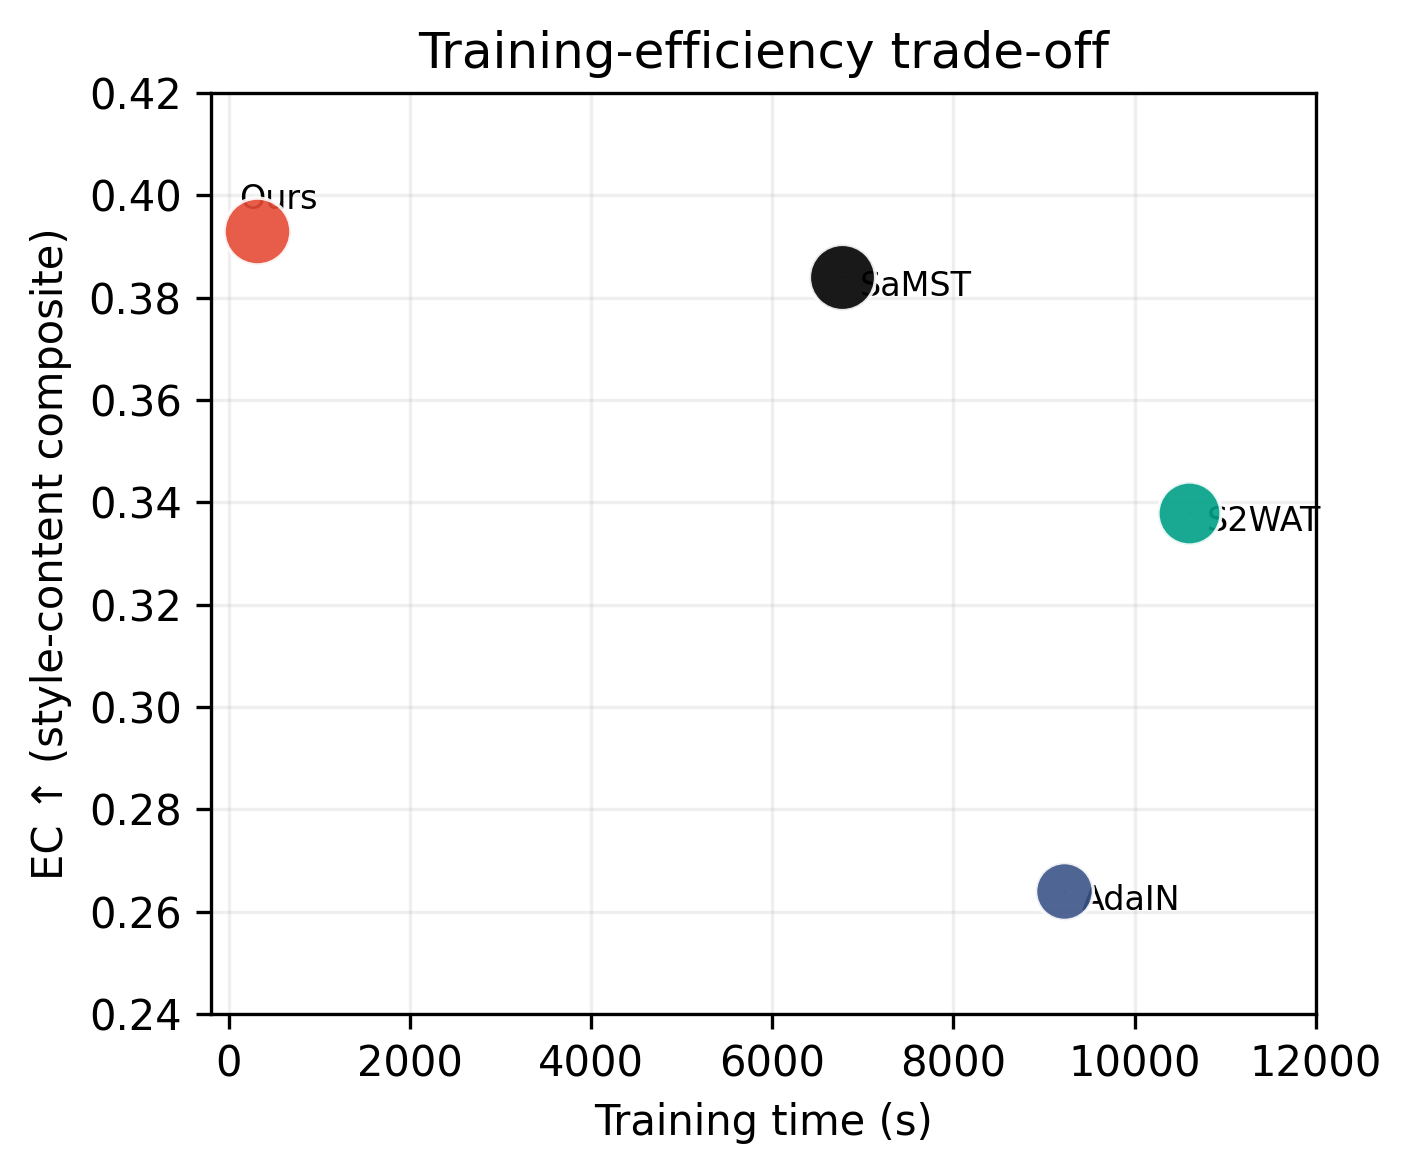
\includegraphics[width=0.82\linewidth]{fig_train_efficiency_pareto.png}
    \caption{训练效率Pareto图（对数刻度）。我们在比较方法中达到最高EC，同时位于最低训练成本区域。标记大小反映参数量。基线训练时间遵循表~\ref{tab:main}中的外推值（$\dagger$）。}
    \label{fig:pareto}
\end{figure}

我们还评估了可选的理论切换。Sinkhorn归一化语义路由和熵门控运动正则化改善EC/内容但降低原始CLIP风格。最佳理论切换EC为熵门控运动，权重5.0第1 epoch，给予CLIP风格0.6916，CLIP内容0.8804，LPIPS 0.3684，EC 0.4368。颜色传输略微提升原始风格但损害LPIPS和内容，因此未被选为主线。

\subsection{步数与$\lambda$敏感性}
额外的步数扫描评估所选第7 epoch检查点的1、4、8、12和16个Euler步骤。主要观察是质量曲线在此范围内几乎平坦。全配对CLIP风格得分仅从0.7159变化至0.7162，而LPIPS保持紧密集中在0.4514左右。Photo转艺术操作点同样稳定：CLIP风格仅从0.6712变化至0.6715，LPIPS保持在0.4881附近。这意味着12步默认不是脆弱的调优最优值。实际上，四步已经恢复几乎相同的质量，而测量的严格750端到端吞吐量从1步的8.43图像/秒增加到4步的9.54图像/秒，并在8—16步保持在约9.34—9.50图像/秒。近似平坦的步曲线表明在所选操作域中学习到的向量场是稳定的，而非表明迭代积分不必要。因此我们保持12步作为保守默认，但扫描表明较低步部署是可行的，当边际延迟减少重要时。

我们还在 $\lambda_{\mathrm{kin}} \in \{0.5, 1.0, 2.0\}$ 和 $\lambda_{\mathrm{swd}} \in \{10, 20, 30\}$ 上扫描 $3 \times 3$ 网格，每个训练8个epoch。结果表面是平滑且可解释的，而非不稳定。增加运动权重同时降低终端压力系统性地改善内容保持：在第8 epoch，设定 $(2.0, 10)$ 给出CLIP内容0.8734，LPIPS 0.3720，EC 0.4373，相比默认 $(1.0, 20)$ 设置的CLIP内容0.8124，LPIPS 0.4477，EC 0.3937。相反，较弱的运动权重或较强的终端权重将模型推向更激进但内容忠实度更低的风格化；例如，$(0.5, 30)$ 将CLIP内容降至0.6926并将LPIPS提高至0.5538。此网格中最佳迁移EC检查点一致地出现在第3 epoch左右，再次表明协议暴露了宽阔的风格—内容前沿而非单一脆弱终点。

\subsection{资源使用与可复现性}
端到端推理和训练时间与主要指标一起列于表~\ref{tab:main}。所有时间在NVIDIA RTX 4070 Laptop GPU（8~GB VRAM）上使用相同的严格750协议测量。标记$\dagger$的训练时间从单epoch探测外推。StyleID按设计是无需训练的。

所有报告的严格750评估使用相同的域协议和预处理流水线。我们还在40轮扫描中评估每个epoch，产出320个检查点评估。仅最终epoch选择可能隐藏风格—内容权衡：K2平衡默认在第3 epoch达到最佳EC，而K1平衡默认在第8 epoch达到最佳原始风格。为改进可复现性，每个训练运行存储解析的运行时配置、源文件快照、检查点和逐epoch CSV日志。Python、NumPy、PyTorch和DataLoader工作线程种子在每次运行中固定。

\section{讨论与局限}
我们不声称在所有方法中最大化原始风格识别；相反，我们声称在高效域级 regime 中具有显著更强的效率—质量权衡。核心结果是LBM保持近SaMST质量（CLIP风格0.716 vs.\ 0.719），改善LPIPS和EC，训练成本降低约$22\times$，并在核心迁移指标上优于更重的S2WAT基线——效率—质量的有利操作点。重要的是，此效率提升并非通过脱离质量前沿而购买：它伴随着比SaMST更好的LPIPS/EC和比S2WAT更强的核心权衡指标。

当前研究仍有若干局限。首先，风格表示是域级而非参考图像特定的；这使推理高效但限制复现独特单图像笔触模式或解决跨域原型冲突的能力。其次，Euler积分故意简单，因此当潜在路径外推到更激进设置或更高分辨率时，离散化误差可能累积。第三，SWD项使用启发式多尺度块投影而非精确传输求解器，因此桥视角应保持有界和实践性而非完全理论性。第四，尽管核心指标和效率分析对于比较基线已完成，但完整伪影诊断包仅针对子集重新运行。感知质量通过伪影敏感诊断而非主观投票评估，符合我们的可复现评估协议。最后，超越当前256基础协议的分辨率泛化仍有待验证。代码和严格750日志将在接受后发布以支持完全可复现性。未来工作应评估更丰富的域原型先验、受控积分范围、更高分辨率外推和更强的偏好导向评估，包括人类或评分标准VLM评估。

\section{结论}
我们提出了用于高效域级艺术迁移的OT耦合潜在流匹配。该方法结合三个互补目标：流匹配损失沿随机潜在桥监督时间条件速度场；终端切片Wasserstein匹配将积分终点拉向目标风格分布；运动正则化约束路径位移以保持内容。在严格的750输出评估下，所得3.9M参数模型达到竞争性CLIP风格（0.716）、高风格方法中最低的LPIPS（0.451）、最佳EC得分（0.393），并显著降低比更重前馈基线的训练成本——域级艺术迁移的Pareto高效操作点。

\FloatBarrier
\bibliography{refs}

\clearpage
\small
\setlength{\itemsep}{1pt}
\setlength{\parskip}{2pt}
\section*{可复现性检查清单}
\noindent\textbf{本文}
\begin{itemize}
\item 包含对所引入AI方法的概要轮廓和/或伪代码描述：\textbf{是}。
\item 明确区分意见、假设和推测与客观事实和结果：\textbf{是}。
\item 为不熟悉读者提供标记清晰的教学参考文献以获得复制所需的背景：\textbf{是}。
\end{itemize}

\noindent\textbf{本文是否做出理论贡献？} \textbf{否}。本文使用有界的桥启发动机而非定理级别的理论声明。

\noindent\textbf{本文是否依赖一个或多个数据集？} \textbf{是}。
\begin{itemize}
\item 提供了选择所进行实验的数据集的动机：\textbf{是}。
\item 本文引入的所有新数据集都包含在数据附录中：\textbf{NA}。
\item 本文引入的所有新数据集将在论文发表时公开可用，并附有允许研究免费使用的许可证：\textbf{NA}。
\item 从现有文献中提取的所有数据集都附有适当的引用：\textbf{是}。
\item 从现有文献中提取的所有数据集都是公开可用的：\textbf{是}。
\item 非公开可用的所有数据集都详细描述，并解释为什么公开替代方案在科学上不令人满意：\textbf{NA}。
\end{itemize}

\noindent\textbf{本文是否包含计算实验？} \textbf{是}。
\begin{itemize}
\item 本文说明了开发论文期间每个（超）参数尝试的次数和值范围，以及用于选择最终参数设置的标准：\textbf{部分}。
\item 预处理数据所需的任何代码都包含在附录中：\textbf{否}。
\item 进行和分析实验所需的所有源代码都包含在代码附录中：\textbf{否}。
\item 进行和分析实验所需的所有源代码将在论文发表时公开可用，并附有允许研究免费使用的许可证：\textbf{部分}。
\item 实现新方法的所有源代码都有注释，详细说明实现，并引用论文中每个步骤的来源：\textbf{部分}。
\item 如果算法依赖随机性，则以足够允许结果复制的方式描述设置种子的方法：\textbf{部分}。
\item 本文指定了用于运行实验的计算基础设施，包括硬件/软件细节：\textbf{部分}。
\item 本文正式描述了使用的评估指标并解释选择这些指标的动机：\textbf{是}。
\item 本文说明了用于计算每个报告结果的算法运行次数：\textbf{是}。
\item 实验分析超越单维性能总结，包括变化、置信度或其他分布信息的度量：\textbf{是}。
\item 使用适当的统计检验判断任何改进或性能下降的意义：\textbf{是}（配对bootstrap，5000次重采样，在实验节中报告）。
\item 本文列出实验中每个模型/算法使用的所有最终（超）参数：\textbf{部分}。
\end{itemize}

\end{document}